\documentclass[11pt,twoside,titlepage]{article}
\usepackage[tc]{titlepic}
\usepackage{times}
\usepackage{float}
\usepackage{amssymb}
\usepackage{amsmath}
\usepackage{amsthm}
\usepackage{needspace}
\usepackage{url}
\usepackage{hyperref}
%\usepackage{mathptm}
\usepackage{fancyhdr}
\usepackage{wrapfig}
\ifx\pdfoutput\undefined
% we are running LaTeX, not pdflatex
\usepackage{epsfig,color}
\else
% we are running pdflatex, so convert .eps files to .pdf
\usepackage[pdftex]{epsfig,color}
\usepackage{epstopdf}
\usepackage{pdfsync}
\fi
\usepackage{ifthen,version}
\usepackage{listings}
%\usepackage{temporal}
%\usepackage{algorithmic}
\newboolean{print-solutions}

% Start of configuration section
% Comment out the following line to exclude the printing of solutions.
%\setboolean{print-solutions}{true}
\newcommand{\labnumber}{1}
\newcommand{\labname}{Digital Logic Gates}
\newcommand{\coursenumber}{Lab Safety How-To Document}
\newcommand{\coursename}{Introduction to Digital Design}
% End of configuration section

% Conditional definitions
\newcommand{\dateorsol}{\LARGE \ifthenelse{\boolean{print-solutions}}%
  {Solutions}{Due \duedate}}
\newcommand{\headertxt}{\sl \ifthenelse{\boolean{print-solutions}}%
  {Solutions to}{} Laboratory Exercise \#\labnumber}
\newcommand{\points}[1]{\ifthenelse{\boolean{print-solutions}}%
  {}{[#1 points.]}}
\ifthenelse{\boolean{print-solutions}}{\includeversion{prnt-solns}}%
{\excludeversion{prnt-solns}}

\textwidth=7.25in
\evensidemargin=-0.35in
\oddsidemargin=-0.35in

\newcommand{\ite}{\operatorname{ite}}
\newcommand{\itec}{\operatorname{ite\_constant}}

{\theoremstyle{definition} \newtheorem{definition}{Definition}}
\newtheorem{theorem}{Theorem}
\newtheorem{lemma}{Lemma}
\newtheorem{corollary}{Corollary}
\newtheorem{proposition}{Proposition}
{\theoremstyle{remark}
  \newtheorem{example}{Example}
  \newtheorem{problem}{Problem}
  \newtheorem{note}{Note}}
% Fortunately, proofs can be nested.
\newenvironment{solution}{\begin{proof}[Solution]}{\end{proof}}


\newcommand{\ta}{Created By: Kyler Scott and Prof. Sunil P. Khatri\\July 2020}
\title{ \huge Department of Electrical and Computer Engineering\\ \huge Texas A\&M University \\}
\author{ \huge Lab Safety:\\ \\ \huge How-To Document \\ \\ \\ \ta}

\titlepic{
\includegraphics[width=0.5\textwidth]{logo}}

\date{}
\pagestyle{fancy}
\lhead[\rm\thepage]{}
\rhead[]{\rm\thepage}
\lfoot[]{\coursenumber}
%\cfoot{\instructor}
\rfoot[\coursenumber]{}

\begin{document}
\bibliographystyle{alpha}
\maketitle

\section{Introduction}
Learning the fundamentals of digital circuits and successfully completing lab assignments will require that you use your lab equipment properly. Before attempting to perform any exercise in any of the ECEN 248 or ECEN 449/749 lab manuals, or in any of the ECEN 248 or ECEN 449/749 how-to documents, you should read and understand this document in full. This document contains important information that will teach you to avoid potential hazards such as destroying your lab equipment or even starting a fire.\\

\section{General Precautions}

\noindent
Do not use any of the materials, components, or equipment present in the "ECEN 248 Lab Parts List" or the "ECEN 449/749 Lab Parts List" for anything other than the intended use. Do not attempt to modify materials, components, or equipment by breaking or bending any part of them, or by removing any protective shielding. Do not use any power supply other than the 5V power adapter present in your lab parts list. When working with the materials, components, or equipment in the lab exercise, do not use any materials, components, or equipment other than those present on your parts list.\\

\noindent
When working with circuits on a breadboard, circuit components will heat up due to the electric current running through them. Usually this will not pose any hazard, but there are instances where the temperature of certain circuit components can become hot enough to cause burns to the skin, to cause a component or your breadboard to melt, or to cause a component or your breadboard to catch fire. To protect yourself and your equipment from these hazards, make sure that any time you are supplying power to your circuit, the breadboard and all circuit components are placed securely on a tabletop or desktop, away from any materials that may be easily flammable and away from any water. Any time you are not using the circuit, the power supply should be turned off and disconnected.\\

\noindent
For similar reasons, it is always a good idea to keep your circuit layout on the breadboard tidy and well organized. Having a crowded circuit with many tangled wires will not only cause you trouble from a troubleshooting perspective, but can increase the likelihood of errors such as misplaced connections, exacerbating the hazards listed above.

\section{LED Precautions}

\noindent
The light emitting diode (LED) components used in ECEN 248 present a safety risk due to their potential to become very hot when powered under certain conditions. You should never wire an LED with more than 2.5V across its electrodes. This can cause the LED to overheat, resulting in the LED being destroyed, melting, or even catching fire. Follow the instructions given in this section to avoid this hazard.\\

\noindent
An LED, as pictured in Figure~\ref{led} is a light source which will emit light if the voltage difference between the anode and cathode is high enough. For the WP7113ID LED used in the 248 labs, this voltage is 2V. In other words, if we connect the cathode to GND, and the anode to a node in our circuit, the LED will light up if the voltage of that node is at least 2V. This 'turn on' voltage for the LED is called the forward voltage. This is useful for the circuits we breadboard, because if VCC$>=$2V, the LED will effectively light up if the node we are measuring is logic '1'.\\

\begin{figure}[!h]
	\centering 
	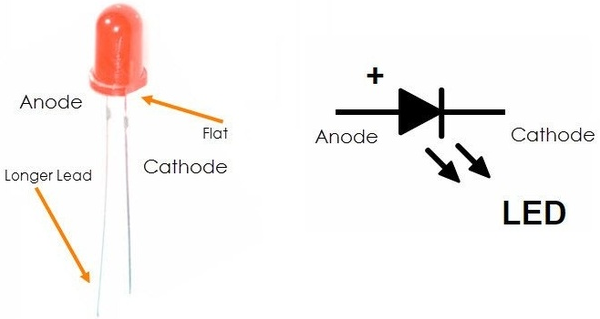
\includegraphics[ width=.5\textwidth]{led}
	\caption{Light Emitting Diode (LED)}
	\label{led}
\end{figure}

\noindent
There is one caution however. If the voltage difference between the anode and cathode is much higher than the forward voltage, the LED can become very hot and can be destroyed or even catch fire. For this reason, we have to take cautions when working on the ECEN 248 and ECEN 449/749 labs, because our VCC is much higher than 2V. This means that if we connect the anode of an LED to a node in our circuit which is logical '1' (about 5V), and the cathode to GND, the LED can easily overheat.\\

\noindent One way we can work around this problem is very simple. Instead of wiring one LED between GND and the node we are measuring, we wire two LEDs in series. This way, there is an intermediate node between GND and VCC where the cathode of the first LED meets the anode of the second, as depicted in Figure~\ref{led2}. This circuit will divide the 5V drop between the two LEDs, so that each LED only has a 2.5V drop over it. 2.5V is above the forward voltage of the LED, so it will light up, but it is not so high that it will overheat. \\

\begin{figure}[!h]
	\centering 
	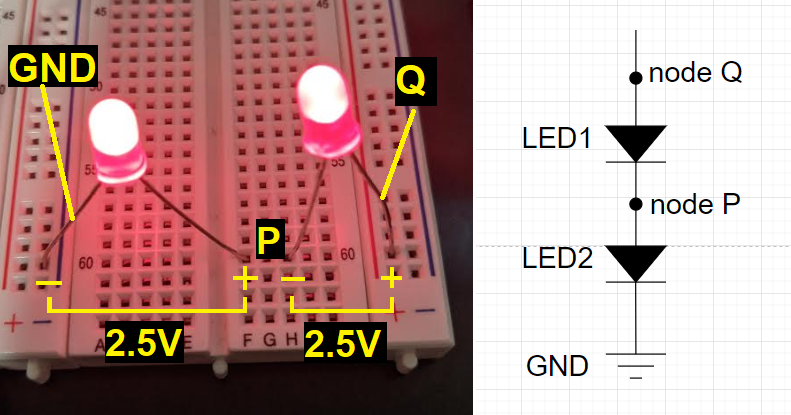
\includegraphics[ width=.6\textwidth]{led2}
	\caption{LED Voltage Divider Circuit}
	\label{led2}
\end{figure}

\noindent
The circuit in Figure~\ref{led2} acts as a simple logic probe, which will tell us if the voltage on a node in our circuit is high (logic 1) or low (logic 0). To create this simple probe circuit, simply wire two LEDs in series, as shown in Figure~\ref{led2}, and connect the cathode of LED2 to GND. Then, connect node Q to  whichever node you wish to measure. If the two LEDs light up, the voltage of the node you are measuring is high (logic 1), and if the two LEDs stay unlit, the node voltage is low (logic 0).\\

\noindent
Every time you use an LED in an ECEN 248 or ECEN 449/749 lab, be sure to use this technique!

\end{document}

